\documentclass[border=3pt]{standalone}
% Preâmbulo compartilhado pelos diagramas TikZ da aula 5 de IHC (Processos de Design)
\usepackage[T1]{fontenc}
\usepackage[utf8]{inputenc}
\usepackage{lmodern}
\usepackage{amsmath}
\usepackage{xcolor}
\usepackage{tikz}
\usetikzlibrary{arrows.meta,angles,quotes,decorations.pathmorphing,calc,
                positioning,shapes.geometric,shapes.misc,backgrounds,fit,
                math}

% Paleta (mesma dos SVGs originais)
% Paleta da disciplina de IHC: acento roxo (#755099), da capa do livro.
% (o nome "dblue" é mantido para não alterar todos os diagramas)
\definecolor{dblue}{HTML}{755099}
\definecolor{dorange}{HTML}{B3541E}
\definecolor{dgreen}{HTML}{4A7C59}
\definecolor{dred}{HTML}{9C4B4B}
\definecolor{dcream}{HTML}{F4F1EA}
\definecolor{dshade}{HTML}{DDD7C9}

% Função gaussiana (não normalizada por padrão de escala visual)
\pgfmathdeclarefunction{gauss}{3}{%
  \pgfmathparse{1/(#3*sqrt(2*pi))*exp(-((#1-#2)^2)/(2*#3^2))}%
}

% Estilos comuns (prefixo d... para não colidir com chaves internas do pgf)
\tikzset{
  >={Stealth[length=2mm]},
  dguide/.style={gray!55, dashed, line width=0.4pt},
  daxis/.style={gray!60, line width=0.7pt, ->},
  dbody/.style={fill=black!3, draw=black!80, line width=1pt},
  dacc/.style={draw=dblue, line width=1pt},
  dlbl/.style={black!55, font=\small},
  dsub/.style={black!45, font=\footnotesize},
  dstate/.style={circle, draw=black!80, fill=dcream, line width=1pt,
                 minimum size=17mm, font=\large, inner sep=1pt},
  dobs/.style={circle, draw=black!80, fill=dshade, line width=1pt,
               minimum size=14mm, font=\large, inner sep=1pt},
  dbox/.style={rounded corners=2pt, draw=black!80, fill=dcream, line width=1pt,
               align=center, inner sep=6pt},
  dop/.style={circle, draw=black!80, fill=white, line width=1pt,
              minimum size=6mm, inner sep=0pt, font=\small},
  dtrans/.style={->, dblue, line width=1pt},
  dmeas/.style={->, dorange, line width=1pt},
  dcurve/.style={line width=1pt, dblue},
  dcurveb/.style={line width=1.4pt, dorange},
}

\begin{document}
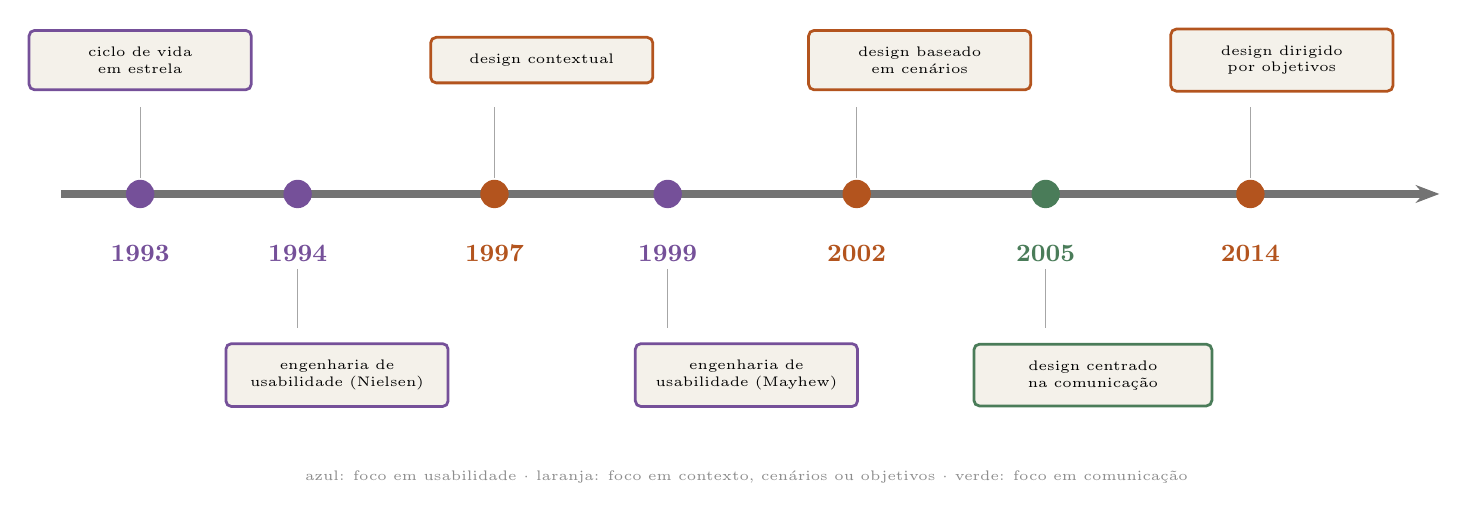
\begin{tikzpicture}[x=1cm,y=1cm]

  \draw[-{Stealth[length=3mm]}, black!55, line width=2.6pt] (-0.5,0) -- (17.0,0);
  \foreach \x/\y/\t/\a/\c in {0.5/1993/{ciclo de vida em estrela}/Hix e Hartson/dblue,
                              2.5/1994/{engenharia de usabilidade}/Nielsen/dblue,
                              5.0/1997/{design contextual}/Beyer e Holtzblatt/dorange,
                              7.2/1999/{engenharia de usabilidade}/Mayhew/dblue,
                              9.6/2002/{design baseado em cenários}/Rosson e Carroll/dorange,
                              12.0/2005/{design centrado na comunicação}/Barbosa et al./dgreen,
                              14.6/2014/{design dirigido por objetivos}/Cooper et al./dorange} {
    \fill[\c] (\x,0) circle (0.18);
    \node[font=\small\bfseries, \c] at (\x,-0.75) {\y};
  }
  \node[dbox, text width=2.4cm, font=\tiny, draw=dblue] at (0.5,1.7) {ciclo de vida em estrela};
  \node[dbox, text width=2.4cm, font=\tiny, draw=dblue] at (3.0,-2.3) {engenharia de usabilidade (Nielsen)};
  \node[dbox, text width=2.4cm, font=\tiny, draw=dorange] at (5.6,1.7) {design contextual};
  \node[dbox, text width=2.4cm, font=\tiny, draw=dblue] at (8.2,-2.3) {engenharia de usabilidade (Mayhew)};
  \node[dbox, text width=2.4cm, font=\tiny, draw=dorange] at (10.4,1.7) {design baseado em cenários};
  \node[dbox, text width=2.6cm, font=\tiny, draw=dgreen] at (12.6,-2.3) {design centrado na comunicação};
  \node[dbox, text width=2.4cm, font=\tiny, draw=dorange] at (15.0,1.7) {design dirigido por objetivos};
  \foreach \x in {0.5,5.0,9.6,14.6} { \draw[black!35] (\x,0.2) -- (\x,1.1); }
  \foreach \x in {2.5,7.2,12.0} { \draw[black!35] (\x,-0.95) -- (\x,-1.7); }
  \node[dsub, font=\tiny] at (8.2,-3.6) {azul: foco em usabilidade $\cdot$ laranja: foco em contexto, cenários ou objetivos $\cdot$ verde: foco em comunicação};

\end{tikzpicture}
\end{document}
